\begin{surferPage}[Labs-Septic]{A Septic with 99 Singularities}
    Oliver Labs constructed a surface of degree $7$ (septic) while working on his
    dissertation at Mainz University in 2004. This is the current world record
    of degree $7$; but there may still exist a septic surface with up to $104$
    singularities!  
    Labs's surface has the symmetry of a regular $7$--gon (left picture).
    This is visible when looking at the surface from the top (right picture):

    \vspace*{-0.3em}
    \begin{center}
      \begin{tabular}{c@{\qquad}c}
        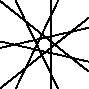
\includegraphics[height=1.5cm]{./../../common/images/labsseptic1.pdf}
        &
        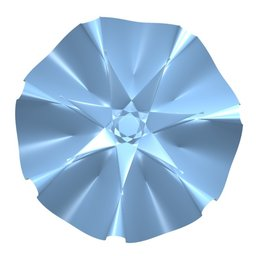
\includegraphics[height=1.5cm]{./../../common/images/labs_septic_von_oben}
      \end{tabular}
    \end{center}
    \vspace*{-0.3em}

    For constructing this surface, Oliver Labs used the computer algebra system
    {\sc Singular} (Kaiserslautern University) which is well suited for
    computations in algebraic geometry and singularities.

    He made use of modular arithmetic. An example of this would be a clock, we know that 24:00$=$0:00, 24:00 $+$ 1 hour is
    not 25:00, but 1:00 o'clock.
\end{surferPage}
